\subsection{Allgemeines}
\label{subsec:pofallgemeines}

Optische Wellenleiter, auch Lichtwellenleiter genannt, verwenden Licht zur
Übertragung von Informationen. Dies ermöglicht eine schnellere Datenübertragung
als mit Kupferkabeln. Glasfaserkabel werden aufgrund ihrer hohen Reichweite von
mehreren Kilometern und der hohen Übertragungsleistung von bis zu 32 Gigabit/s
pro Kabel für die Verbindung von Städten und Kontinenten eingesetzt. Die
Anbindung von Gebäuden und Wohnungen an das Glasfaserkabelnetz ist mittlerweile
ein erklärtes Ziel der Telekommunikationsunternehmen. Durch Projekte wie \glqq
Fiber to the Home\grqq{} oder \glqq Fiber to the Building\grqq{} sollen
Privatpersonen und Unternehmen von hohen Übertragungsgeschwindigkeiten
profitieren. Für die Verlegung in Gebäuden sind Glasfaserkabel jedoch nur
bedingt geeignet, da Fachpersonal mit Spezialwerkzeug erforderlich ist. Polymer
optische Fasern (POF) bieten sich hier als kostengünstige Alternative an. Sie
lassen sich einfach und platzsparend verlegen (der Durchmesser beträgt ca. 1 mm)
und auf kurzen Distanzen \nolbreaks{(< 100 m)} können Datenraten von bis zu 40
Gigabit/s erreicht werden \cite{pofacgif}. Kabel aus polymer optischen Fasern
werden außerdem in Flugzeugen, Zügen, Automobilen und Industrieanlagen
eingesetzt. \autoref{fig:pofgrund} zeigt die Gründe für die Verwendung in dem
jeweiligen Bereich. Die Größe des Kreises in der jeweiligen Zelle gibt die
Relevanz des Kriteriums an. \cite{poflan}

\ifthenelse{\boolean{showPics}}{
    \begin{figure}[h]
        \begin{center}
            \begin{minipage}[t]{\textwidth}
                \begin{center}
                    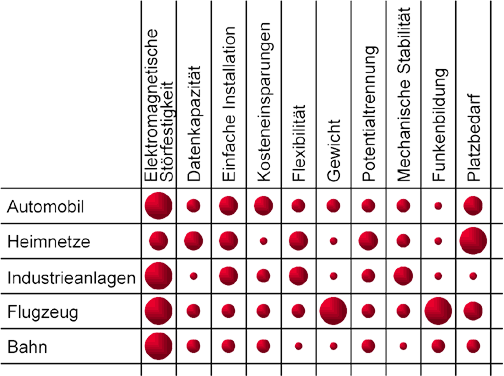
\includegraphics[height=0.2\textheight]{Bilder/Optische_Wellenleiter_Die_Polymer_Optische_Faser/Allgemeines/pofgrund.png}
                    \caption[Gründe für die Verwendung von POF-Kabel \newline \url{http://www.pofac.fh-nuernberg.de/pofac/de/was_sind_pof/images/warum_pof.png} (zuletzt aufgerufen am 19.09.2015)]{Gründe für die Verwendung von POF-Kabel}
                    \label{fig:pofgrund}
                \end{center}
            \end{minipage}
        \end{center}
    \end{figure}
}{}

Elektromagnetische Strahlung, elektrische Felder und Magnetfelder
beeinträchtigen den Fluss von Elektronen in Kupferkabeln, jedoch nicht den von
Lichtstrahlen in einem Lichtwellenleiter. Daher kommen polymer optische Fasern
überall dort zum Einsatz, wo eine ungestörte Datenübertragung wichtig ist. In
Flugzeugen reduziert das geringe Gewicht von POF-Kabeln den Treibstoffverbrauch
und damit die Betriebskosten. Zudem wird Funkenbildung vermieden, da polymer
optische Fasern keine Elektronen sondern Licht übertragen. POF-Kabel werden auch
in Krankenhäusern eingesetzt, da sie keine elektromagnetische Strahlung
emittieren und deshalb empfindliche Messgeräte nicht stören.
